\documentclass{article}
\usepackage{graphicx}
\usepackage{subcaption}
\usepackage{caption}
\usepackage{wrapfig}  % For wrapping text around figures
\usepackage{float}    % For precise figure placement
\usepackage{tikz}     % For drawing diagrams

% Title Page
\title{LaTeX Workshop: Figures}
\author{
    \begin{tabular}{c c c}
        Dalia Kamalzadeh & \hspace{2cm} & Koorosh Komeili Zadeh \\
        Student Mentor & & Student Mentor \\
        Universiteit Leiden & & Universiteit Leiden
    \end{tabular}
}
\date{}
\begin{document}
\maketitle

\section*{Including Figures in LaTeX}

To insert images in LaTeX, use the \texttt{graphicx} package. Here’s how to do it:

\begin{verbatim}
\begin{figure}[h]
    \centering
    \includegraphics[width=0.7\textwidth]{image.png}
    \caption{A sample image}
\end{figure}
\end{verbatim}

\subsection*{Side-by-Side Figures}

You can place multiple images side-by-side using the \texttt{subcaption} package:

\begin{figure}[h]
    \centering
    \begin{subfigure}{0.45\textwidth}
        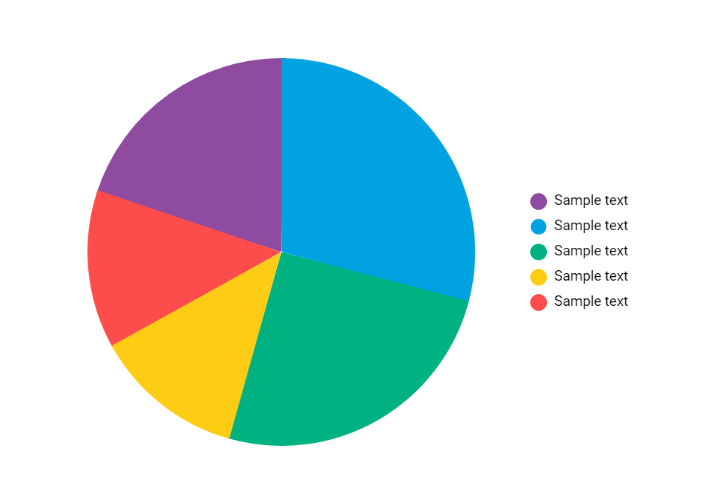
\includegraphics[width=\linewidth]{Figures/sample-pie.png}
        \caption{First Image}
    \end{subfigure}
    \begin{subfigure}{0.45\textwidth}
        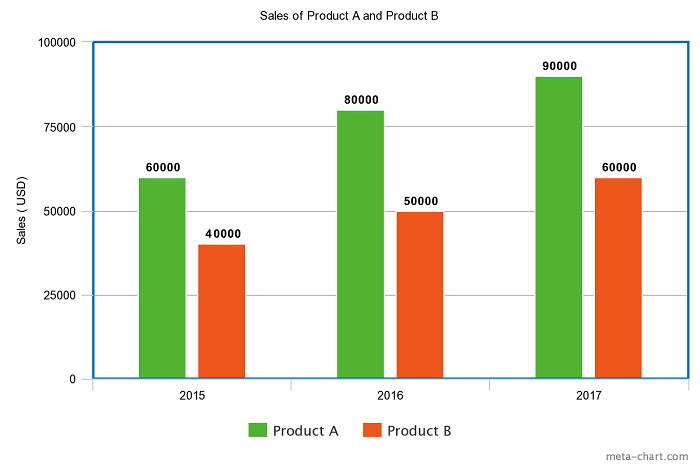
\includegraphics[width=\linewidth]{Figures/sample-bar.png}
        \caption{Second Image}
    \end{subfigure}
    \caption{Two charts side-by-side}
\end{figure}

\subsection*{Resizing and Rotating Images}

You can resize or rotate images easily using the \texttt{graphicx} package. Here are examples of resizing and rotating an image:

\textbf{Resizing an Image:}
\begin{verbatim}
\includegraphics[width=0.5\textwidth]{image.png}
\end{verbatim}

\textbf{Rotating an Image:}
\begin{verbatim}
\includegraphics[angle=90, width=0.5\textwidth]{image.png}
\end{verbatim}

Example of a rotated image:
\begin{figure}[h]
    \centering
    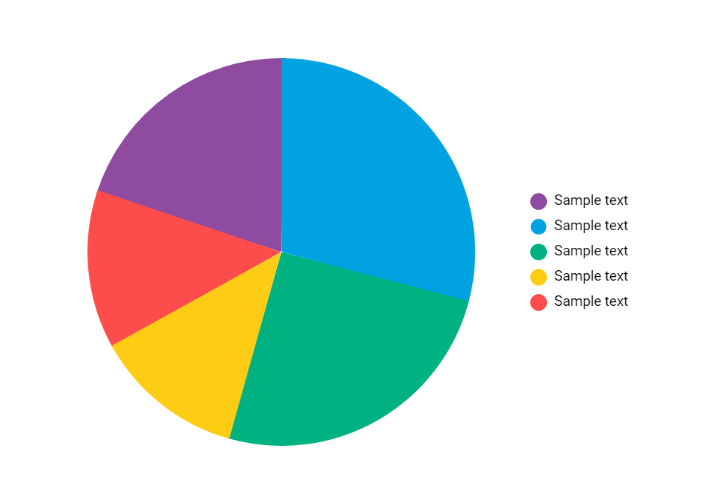
\includegraphics[angle=90, width=0.5\textwidth]{Figures/sample-pie.png}
    \caption{Rotated Image by 90 degrees}
\end{figure}

\subsection*{Wrapping Text Around Figures}

Sometimes you may want text to flow around an image. You can use the \texttt{wrapfig} package to achieve this:

\begin{wrapfigure}{r}{0.4\textwidth}
    \centering
    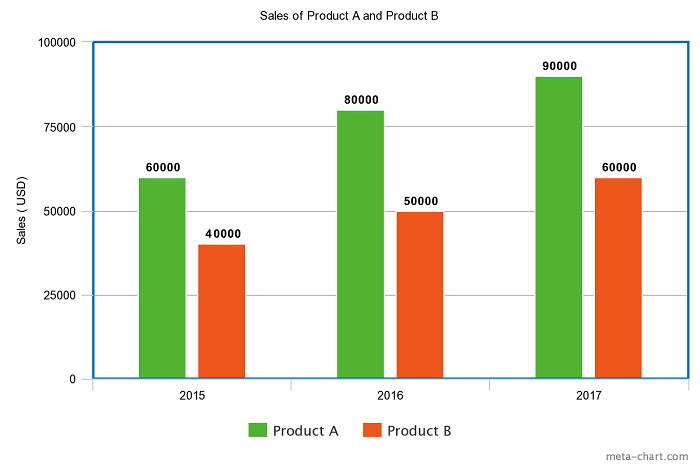
\includegraphics[width=0.4\textwidth]{Figures/sample-bar.png}
    \caption{Wrapped Figure}
\end{wrapfigure}

This figure is wrapped with text flowing around it. You can adjust the position and size of the figure using the \texttt{wrapfig} package.

\subsection*{Using External Images from URLs}

You can also include images from URLs using the \texttt{graphicx} package, although this requires special support from Overleaf or other online compilers:

\begin{verbatim}
\includegraphics[width=0.5\textwidth]{https://example.com/image.png}
\end{verbatim}

\subsection*{Creating Diagrams with TikZ}

LaTeX also allows you to create vector graphics natively using the \texttt{TikZ} package. Here's a simple example of drawing a circle with text inside it:

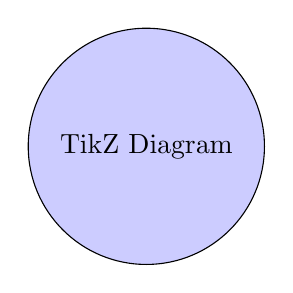
\begin{tikzpicture}
    \draw[fill=blue!20] (0,0) circle [radius=1.5] node {TikZ Diagram};
\end{tikzpicture}

You can create much more complex diagrams, flowcharts, and shapes with TikZ, which is very powerful for vector-based graphics.

\subsection*{Floating Figures and Exact Placement}

Sometimes, you may want precise control over figure placement. The \texttt{float} package allows you to use the \texttt{H} option to force a figure to appear exactly where you specify in the document:

\begin{verbatim}
\begin{figure}[H] % Use 'H' to force the figure here
    \centering
    \includegraphics[width=0.6\textwidth]{image.png}
    \caption{Forced Figure Placement}
\end{figure}
\end{verbatim}

\subsection*{Subfigures with Different Captions}

You can create a single figure with multiple images (subfigures) using the \texttt{subcaption} package:

\begin{figure}[h]
    \centering
    \begin{subfigure}{0.4\textwidth}
        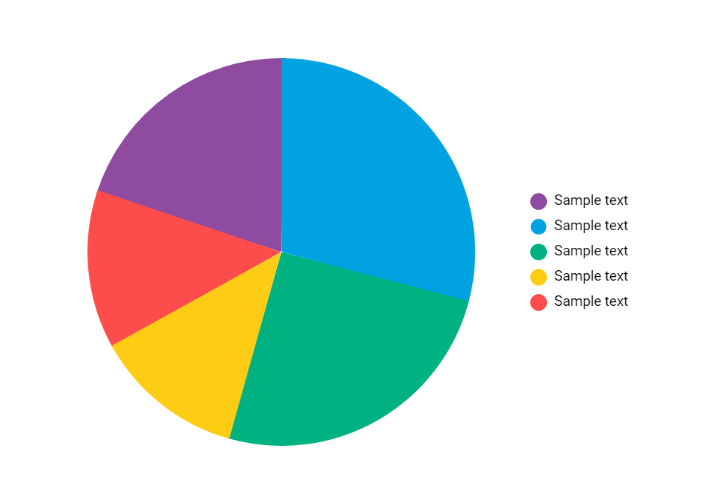
\includegraphics[width=\linewidth]{Figures/sample-pie.png}
        \caption{Pie Chart}
    \end{subfigure}
    \hspace{0.05\textwidth} % Add some space between figures
    \begin{subfigure}{0.4\textwidth}
        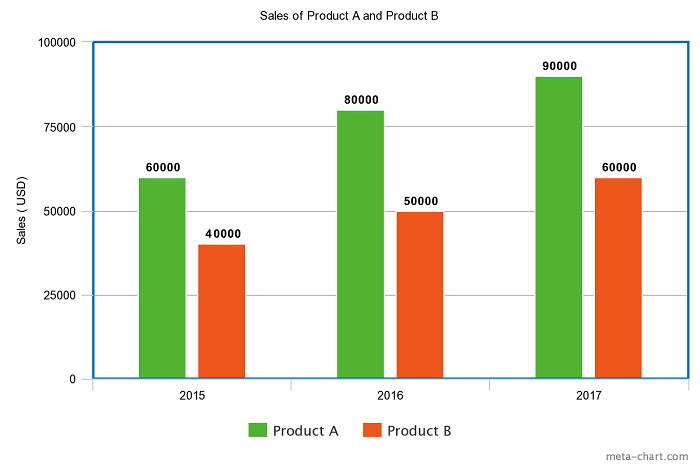
\includegraphics[width=\linewidth]{Figures/sample-bar.png}
        \caption{Bar Chart}
    \end{subfigure}
    \caption{Comparison between Pie and Bar Charts}
\end{figure}

\end{document}
